\documentclass[12pt,a4paper]{article}

% ─── Page Layout ───────────────────────────────────────────────────────────────
\usepackage[a4paper, margin=0.8in, headheight=14pt]{geometry}

% ─── Fonts (XeLaTeX) ───────────────────────────────────────────────────────────
\usepackage{fontspec}
\usepackage{unicode-math}
\setmainfont{TeX Gyre Pagella}
\setmonofont[Scale=0.88]{TeX Gyre Cursor}
\setmathfont{Latin Modern Math}

% ─── Packages ──────────────────────────────────────────────────────────────────
\usepackage{xcolor}
\usepackage{colortbl}
\usepackage{titlesec}
\usepackage{enumitem}
\usepackage{tabularx}
\usepackage{booktabs}
\usepackage{array}
\usepackage{amsmath}
\usepackage{tikz}
\usetikzlibrary{shapes.geometric, arrows.meta, positioning, calc, fit, decorations.pathreplacing, patterns}
\usepackage{tcolorbox}
\tcbuselibrary{skins, breakable}
\usepackage{hyperref}
\usepackage{fancyhdr}
\usepackage{graphicx}
\usepackage{microtype}
\hyphenpenalty=10000
\exhyphenpenalty=10000
\sloppy
\usepackage{caption}
\usepackage{setspace}
\usepackage{multirow}
\usepackage{tocloft}

% ─── Q&A helper ────────────────────────────────────────────────────────────────
\newcommand{\Q}[1]{\textbf{#1}\par\noindent\ignorespaces}

% ─── Colour Palette ────────────────────────────────────────────────────────────
\definecolor{myred}{RGB}{196,30,58}
\definecolor{mydark}{RGB}{30,30,50}
\definecolor{mygreen}{RGB}{14,120,80}
\definecolor{myteal}{RGB}{0,130,140}
\definecolor{myamber}{RGB}{180,100,0}
\definecolor{mypurple}{RGB}{100,30,160}
\definecolor{mygray}{RGB}{246,247,249}
\definecolor{mgframe}{RGB}{180,185,200}
\definecolor{watermark}{RGB}{145,150,170}
\definecolor{hdrred}{RGB}{250,232,235}
\definecolor{hdrgreen}{RGB}{220,244,233}
\definecolor{hdrteal}{RGB}{220,242,244}
\definecolor{hdramber}{RGB}{253,242,215}
\definecolor{hdrpurple}{RGB}{238,228,255}
\definecolor{hdrgray}{RGB}{238,240,245}
\definecolor{rowalt}{RGB}{250,251,253}

% ─── Section Formatting ────────────────────────────────────────────────────────
\titleformat{\section}
  {\large\bfseries\color{myred}}{\thesection.}{0.5em}{}
  [\vspace{1pt}{\color{myred}\rule{\linewidth}{0.8pt}}]
\titleformat{\subsection}
  {\normalsize\bfseries\color{myteal}}{\thesubsection}{0.5em}{}
\titlespacing*{\section}{0pt}{18pt}{7pt}
\titlespacing*{\subsection}{0pt}{11pt}{4pt}

% ─── Paragraph ─────────────────────────────────────────────────────────────────
\setlength{\parindent}{0pt}
\setlength{\parskip}{4pt}

% ─── TOC Styling ───────────────────────────────────────────────────────────────
\renewcommand{\cfttoctitlefont}{\large\bfseries\color{myred}}
\renewcommand{\cftaftertoctitle}{\par\noindent{\color{myred}\rule{\linewidth}{0.8pt}}}
\setlength{\cftbeforetoctitleskip}{0pt}
\setlength{\cftaftertoctitleskip}{6pt}
\renewcommand{\cftsecfont}{\normalsize\bfseries\color{mydark}}
\renewcommand{\cftsecpagefont}{\normalsize\bfseries\color{mydark}}
\renewcommand{\cftsecleader}{\cftdotfill{\cftdotsep}}
\setlength{\cftbeforesecskip}{7pt}
\renewcommand{\cftsubsecfont}{\small\color{mydark}}
\renewcommand{\cftsubsecpagefont}{\small\color{mydark}}
\setlength{\cftbeforesubsecskip}{3pt}
\setlength{\cftsubsecindent}{1.4em}

% ─── Table helpers ─────────────────────────────────────────────────────────────
\renewcommand{\arraystretch}{1.45}
\setlength{\tabcolsep}{6pt}
\arrayrulecolor{mydark}
\newcolumntype{B}[1]{>{\small\bfseries\raggedright\arraybackslash}m{#1}}
\newcolumntype{Y}{>{\small\raggedright\arraybackslash}X}
\renewcommand{\tabularxcolumn}[1]{m{#1}}

% ─── Header / Footer ───────────────────────────────────────────────────────────
\pagestyle{fancy}
\fancyhf{}
\fancyhead[L]{\small\color{myred}\textbf{EC302}\;\color{mydark}--- Digital System Design}
\fancyhead[R]{\small\color{myteal}\textbf{Module 2 Notes}}
\fancyfoot[C]{\small\color{mydark}\thepage}
\fancyfoot[R]{\small\color{watermark}\textit{\copyright\ Biraj}}
\renewcommand{\headrulewidth}{0.5pt}
\renewcommand{\footrulewidth}{0.3pt}

% ─── Hyperref ──────────────────────────────────────────────────────────────────
\hypersetup{
  colorlinks=true, linkcolor=myteal, urlcolor=myteal,
  pdfauthor={Biraj Sarkar (CGEC)},
  pdftitle={EC302 --- Module 2 Notes: Sequential Logic Design, Counters, and FSM}
}

% ─── tcolorbox styles ──────────────────────────────────────────────────────────
\tcbset{
  tikzbox/.style={
    colback=mygray, colframe=mgframe, boxrule=0.6pt, arc=4pt,
    left=8pt, right=8pt, top=6pt, bottom=6pt,
    colbacktitle=mgframe, coltitle=mydark,
    fonttitle=\small\bfseries
  },
  defbox/.style={
    colback=hdrgreen, colframe=mygreen, boxrule=0.8pt, arc=4pt,
    left=9pt, right=9pt, top=6pt, bottom=6pt,
    colbacktitle=mygreen, coltitle=white,
    fonttitle=\small\bfseries
  },
  formulabox/.style={
    colback=hdrteal, colframe=myteal, boxrule=0.8pt, arc=4pt,
    left=9pt, right=9pt, top=6pt, bottom=6pt,
    colbacktitle=myteal, coltitle=white,
    fonttitle=\small\bfseries
  },
  examplebox/.style={
    colback=hdramber, colframe=myamber, boxrule=0.8pt, arc=4pt,
    left=9pt, right=9pt, top=6pt, bottom=6pt,
    colbacktitle=myamber, coltitle=white,
    fonttitle=\small\bfseries
  },
  masonbox/.style={
    colback=hdrpurple, colframe=mypurple, boxrule=0.8pt, arc=4pt,
    left=9pt, right=9pt, top=6pt, bottom=6pt,
    colbacktitle=mypurple, coltitle=white,
    fonttitle=\small\bfseries
  },
  exambox/.style={
    colback=hdrpurple, colframe=mypurple, boxrule=1pt, arc=5pt,
    left=10pt, right=10pt, top=8pt, bottom=8pt,
    colbacktitle=mypurple, coltitle=white,
    fonttitle=\bfseries,
    breakable, title after break={\textbf{Frequently Asked / Viva Questions (contd.)}}
  }
}

\tcbset{after={\color{black}}}

% ─── TikZ styles ───────────────────────────────────────────────────────────────
\tikzset{
  ffblock/.style={rectangle, draw=myteal, fill=hdrteal,
    minimum width=2.0cm, minimum height=2.4cm,
    font=\small\bfseries, rounded corners=3pt, line width=0.8pt, align=center},
  combblock/.style={rectangle, draw=mypurple, fill=hdrpurple,
    minimum width=2.4cm, minimum height=1.6cm,
    font=\small\bfseries, rounded corners=3pt, line width=0.8pt, align=center},
  state/.style={circle, draw=myteal, fill=hdrteal,
    minimum size=1.0cm, font=\small\bfseries, line width=0.8pt, align=center},
  flowarrow/.style={-Stealth, thick, color=mydark}
}

\begin{document}

% ─── Title Page ───────────────────────────────────────────────────────────────
\begin{titlepage}
  \centering
  \vspace*{1.5cm}
  {\Huge\bfseries\color{myred} Digital System Design\par}
  \vspace{0.4cm}
  {\LARGE\bfseries\color{myteal} Module 2 --- Sequential Logic Design, Counters, and Finite State Machines\par}
  \vspace{0.8cm}
  {\large\textbf{Course Code:} EC302 \;\textbar\; \textbf{Semester:} 3rd Semester (ECE)\par}
  \vspace{0.2cm}
  {\large MAKAUT B.Tech Maulana Abul Kalam Azad University of Technology\par}
  \vspace{1.5cm}
  \begin{tcolorbox}[tikzbox, width=0.85\linewidth]
    \centering
    \textbf{\color{myred}Author:} Biraj Sarkar \;\textbar\; Cooch Behar Government Engineering College\\
    \small Comprehensive, exam-ready lecture notes covering Latches, Flip-Flops, Race-Around Condition, Master-Slave JK, Ripple and Synchronous Counters, Shift Registers, Mealy/Moore FSMs, and PRBS/LFSR Generators.
  \end{tcolorbox}
  \vfill
  {\small\color{watermark} \copyright\ Biraj Sarkar \;\textbar\; Academic Non-Commercial Notes \;\textbar\; CC BY-NC-SA 4.0\par}
\end{titlepage}

\tableofcontents
\newpage

% ===============================================================================
\section{Latches and Flip-Flops}
% ===============================================================================

In sequential logic circuits, outputs depend not only on current inputs but also on past history stored in memory elements.

\subsection{Latches vs. Flip-Flops}
\begin{itemize}[leftmargin=*, itemsep=3pt]
  \item \textbf{Latch:} A level-triggered bistable storage device that responds continuously to inputs whenever the enable/clock signal is at an active level (transparent).
  \item \textbf{Flip-Flop:} An edge-triggered storage device that samples inputs and updates outputs only at a discrete transition (positive rising edge $\uparrow$ or negative falling edge $\downarrow$) of the clock signal.
  \item \textbf{Setup Time ($t_s$):} The minimum time for which the data input must remain stable \textit{before} the arrival of the active clock edge.
  \item \textbf{Hold Time ($t_h$):} The minimum time for which the data input must remain stable \textit{after} the active clock edge.
  \item \textbf{Metastability:} An unstable intermediate output voltage state occurring if setup or hold times are violated.
\end{itemize}

\subsection{The S-R Latch and Forbidden State}
An S-R (Set-Reset) latch constructed with cross-coupled NOR gates operates as follows:
\begin{itemize}[leftmargin=*, itemsep=3pt]
  \item $S=0, R=0 \implies Q_{n+1} = Q_n$ (No change / Hold state).
  \item $S=0, R=1 \implies Q_{n+1} = 0, \overline{Q}_{n+1} = 1$ (Reset state).
  \item $S=1, R=0 \implies Q_{n+1} = 1, \overline{Q}_{n+1} = 0$ (Set state).
  \item $S=1, R=1 \implies Q = \overline{Q} = 0$ (\textbf{Invalid / Forbidden State}). When both inputs simultaneously drop from $1$ to $0$, the circuit enters a race condition, settling into an unpredictable state.
\end{itemize}

\subsection{J-K Flip-Flop and the Race-Around Condition}
The J-K flip-flop eliminates the invalid state of the S-R flip-flop by feeding back outputs $Q$ and $\overline{Q}$ to the input AND gates:
\begin{equation}
  S = J \cdot \overline{Q}, \qquad R = K \cdot Q
\end{equation}
When $J = K = 1$, the flip-flop toggles its output on each active clock: $Q_{n+1} = \overline{Q}_n$.

\begin{tcolorbox}[defbox, title={\textbf{The Race-Around Condition in Level-Triggered JK Flip-Flops}}]
\textbf{Definition:} In a level-triggered JK flip-flop, when $J = K = 1$ and the clock pulse width $t_w$ is greater than the propagation delay $t_{pd}$ of the flip-flop ($t_{pd} < t_w$), the output toggles repeatedly and uncontrollably back and forth ($0 \to 1 \to 0 \to 1 \dots$) during the single high clock interval. At the end of the clock pulse, the final state of $Q$ is indeterminate.

\textbf{Mathematical Condition for Race-Around:}
\begin{equation}
  t_{pd} < t_w < \frac{T}{2}
\end{equation}
where $T$ is the clock period and $t_w$ is the pulse duration.

\textbf{Methods to Prevent Race-Around:}
\begin{enumerate}[label=\alph*., leftmargin=*]
  \item \textbf{Edge Triggering:} Design the circuit to respond only to steep clock transitions ($t_w \approx 0$).
  \item \textbf{Propagation Delay Control:} Choose components such that $t_{pd} > t_w$ (difficult and limits maximum operating frequency).
  \item \textbf{Master-Slave JK Flip-Flop Configuration:} The universal and standard architecture.
\end{enumerate}
\end{tcolorbox}

\subsection{Master-Slave JK Flip-Flop Architecture}
The Master-Slave JK flip-flop consists of two cascaded latches clocked on complementary phases:
\begin{itemize}[leftmargin=*, itemsep=3pt]
  \item \textbf{Master Latch:} Enabled when $\text{CLK} = 1$. It samples inputs $J$ and $K$ and updates its intermediate state ($Q_M$). The Slave latch remains disabled (isolated) because $\overline{\text{CLK}} = 0$.
  \item \textbf{Slave Latch:} When the clock falls ($\text{CLK} = 0 \implies \overline{\text{CLK}} = 1$), the Master is disabled, locking its state. The Slave is enabled and copies the state $Q_M$ to the final external output $Q$.
  \item Because the output $Q$ updates only on the clock falling edge when the Master is completely disabled, feedback cannot affect the Master during the same clock cycle, \textbf{completely eliminating race-around}.
\end{itemize}

\begin{tcolorbox}[tikzbox, title={Master-Slave JK Flip-Flop Functional Architecture}]
\centering
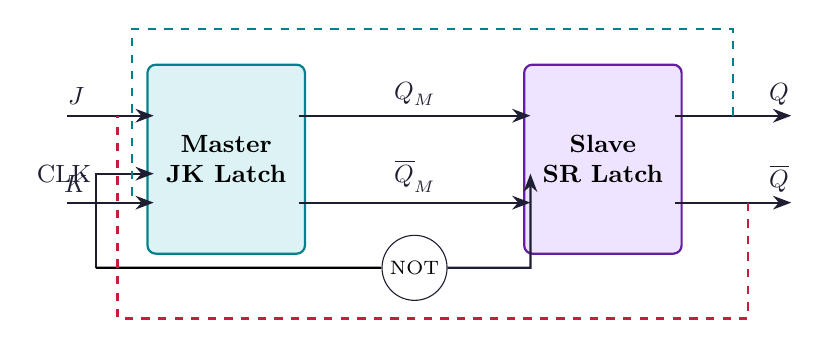
\begin{tikzpicture}[scale=0.92]
  % Master Box
  \node[ffblock, draw=myteal, fill=hdrteal] (master) at (0, 0) {Master\\JK Latch};
  % Inverter
  \node[draw=mydark, circle, inner sep=2pt, font=\scriptsize] (inv) at (2.6, -1.5) {$\text{NOT}$};
  % Slave Box
  \node[ffblock, draw=mypurple, fill=hdrpurple] (slave) at (5.2, 0) {Slave\\SR Latch};

  % Inputs
  \draw[flowarrow] (-2.2, 0.6) -- (-1.0, 0.6) node[pos=0.1, above, font=\small] {$J$};
  \draw[flowarrow] (-2.2, -0.6) -- (-1.0, -0.6) node[pos=0.1, above, font=\small] {$K$};

  % Clock distribution
  \draw[flowarrow] (-1.8, -1.5) -- (-1.8, -0.2) -- (-1.0, -0.2) node[pos=0.1, left, font=\small] {$\text{CLK}$};
  \draw[thick] (-1.8, -1.5) -- (inv);
  \draw[flowarrow] (inv) -- (4.2, -1.5) -- (4.2, -0.2);

  % Interconnect
  \draw[flowarrow] (1.0, 0.6) -- (4.2, 0.6) node[midway, above, font=\small] {$Q_M$};
  \draw[flowarrow] (1.0, -0.6) -- (4.2, -0.6) node[midway, above, font=\small] {$\overline{Q}_M$};

  % Outputs
  \draw[flowarrow] (6.2, 0.6) -- (7.8, 0.6) node[pos=0.9, above, font=\small] {$Q$};
  \draw[flowarrow] (6.2, -0.6) -- (7.8, -0.6) node[pos=0.9, above, font=\small] {$\overline{Q}$};

  % Feedback paths
  \draw[thick, dashed, color=myred] (7.2, -0.6) -- (7.2, -2.2) -- (-1.5, -2.2) -- (-1.5, 0.6);
  \draw[thick, dashed, color=myteal] (7.0, 0.6) -- (7.0, 1.8) -- (-1.3, 1.8) -- (-1.3, -0.6);
\end{tikzpicture}
\end{tcolorbox}

\subsection{Characteristic Equations and Excitation Tables}
\par\vspace{6pt}\noindent
\begingroup
\setlength{\tabcolsep}{3.5pt}
\setlength{\extrarowheight}{3pt}
\renewcommand{\arraystretch}{1.35}
\begin{tabularx}{\linewidth}{|B{1.6cm}|B{3.2cm}|Y|Y|Y|Y|}
\hline
\textbf{Type} & \textbf{Characteristic Equation} & \textbf{$Q_n \to Q_{n+1}$: $0 \to 0$} & \textbf{$0 \to 1$} & \textbf{$1 \to 0$} & \textbf{$1 \to 1$} \\
\hline
S-R & $Q_{n+1} = S + \overline{R} Q_n$ ($S R = 0$) & $S=0, R=X$ & $S=1, R=0$ & $S=0, R=1$ & $S=X, R=0$ \\
\hline
J-K & $Q_{n+1} = J \overline{Q}_n + \overline{K} Q_n$ & $J=0, K=X$ & $J=1, K=X$ & $J=X, K=1$ & $J=X, K=0$ \\
\hline
D & $Q_{n+1} = D$ & $D = 0$ & $D = 1$ & $D = 0$ & $D = 1$ \\
\hline
T & $Q_{n+1} = T \oplus Q_n$ & $T = 0$ & $T = 1$ & $T = 1$ & $T = 0$ \\
\hline
\end{tabularx}
\endgroup

% ===============================================================================
\section{Registers and Shift Registers}
% ===============================================================================

An $n$-bit register is a cascade of $n$ flip-flops sharing a common clock, designed to store and shift multi-bit binary data words.

\subsection{Shift Register Configurations}
\begin{itemize}[leftmargin=*, itemsep=3pt]
  \item \textbf{SISO (Serial-In Serial-Out):} Data enters one bit per clock cycle and exits serially. Requires $n$ clock cycles to load and $n$ clock cycles to read an $n$-bit word.
  \item \textbf{SIPO (Serial-In Parallel-Out):} Data enters serially; all $n$ bits are accessible simultaneously on parallel outputs after $n$ clock cycles.
  \item \textbf{PISO (Parallel-In Serial-Out):} Data is loaded into all flip-flops simultaneously in a single clock cycle using parallel load gates, then shifted out serially.
  \item \textbf{PIPO (Parallel-In Parallel-Out):} Parallel loading and parallel output reading simultaneously in $1$ clock cycle.
\end{itemize}

\subsection{Universal Shift Register (IC 74194)}
A bidirectional 4-bit Universal Shift Register can perform all four data transfer operations controlled by two mode select inputs $S_1, S_0$:
\begin{equation}
  S_1 S_0 = 00 \implies \text{Hold}, \quad 01 \implies \text{Shift Right}, \quad 10 \implies \text{Shift Left}, \quad 11 \implies \text{Parallel Load}
\end{equation}

% ===============================================================================
\section{Asynchronous (Ripple) and Synchronous Counters}
% ===============================================================================

A counter is a specialized sequential circuit that cycles through a prescribed sequence of binary states upon receiving clock pulses.

\subsection{Asynchronous (Ripple) Counters}
In a ripple counter, the external clock is applied \textbf{only to the first flip-flop (LSB)}. Each subsequent flip-flop is clocked by the output of the preceding stage ($Q$ or $\overline{Q}$).
\begin{itemize}[leftmargin=*, itemsep=3pt]
  \item \textbf{Up-Counter vs. Down-Counter:}
    \begin{itemize}
      \item Negative edge-triggered FF with clock connected to $Q_i \implies$ Up-counter.
      \item Negative edge-triggered FF with clock connected to $\overline{Q}_i \implies$ Down-counter.
    \end{itemize}
  \item \textbf{Mod-N Ripple Counter:} Formed by resetting all flip-flops using an active-low asynchronous clear ($\overline{\text{CLR}}$) driven by a NAND gate when the count reaches state $N$.
  \item \textbf{Disadvantages of Ripple Counters:}
    \begin{enumerate}
      \item Accumulated delay: Total propagation delay is $t_{\text{total}} = n \times t_{pd}$.
      \item Maximum operating frequency is constrained: $f_{\text{max}} \le \frac{1}{n \cdot t_{pd}}$.
      \item Transient false counting states (glitches) appear on outputs during transition intervals.
    \end{enumerate}
\end{itemize}

\subsection{Synchronous Counters}
In a synchronous counter, the master clock is connected \textbf{in parallel to all flip-flops simultaneously}. State transitions occur at the exact same clock instant.

\textbf{Systematic Synchronous Counter Design Procedure:}
\begin{enumerate}[label=\arabic*., leftmargin=*]
  \item Determine number of flip-flops: $2^n \ge N$.
  \item Construct the State Transition Diagram and State Table.
  \item Substitute flip-flop excitation requirements ($J_i, K_i$ or $T_i$ or $D_i$) from the excitation table.
  \item Minimize excitation expressions using Karnaugh maps.
  \item Implement the logic circuit.
\end{enumerate}

\subsection{Ring Counter and Johnson (Twisted Ring) Counter}
\begin{itemize}[leftmargin=*, itemsep=3pt]
  \item \textbf{Ring Counter:} An $n$-bit shift register with true output $Q_n$ fed back to serial input $D_1$. A single circulating '1' ($1000 \to 0100 \to 0010 \to 0001$).
    \begin{equation}
      \text{Number of unique states} = n, \qquad \text{Unused states} = 2^n - n
    \end{equation}
  \item \textbf{Johnson (Twisted Ring) Counter:} An $n$-bit shift register with inverted output $\overline{Q}_n$ fed back to $D_1$.
    \begin{equation}
      \text{Number of unique states} = 2n, \qquad \text{Unused states} = 2^n - 2n
    \end{equation}
    Requires only simple 2-input AND gates for complete glitch-free state decoding.
\end{itemize}

% ===============================================================================
\section{Finite State Machines (FSM)}
% ===============================================================================

Any synchronous sequential circuit can be modeled formally as a Finite State Machine consisting of combinational logic and state memory registers.

\subsection{Mealy vs. Moore FSM Models}
\begin{tcolorbox}[defbox, title={\textbf{Architectural Definitions of Mealy and Moore Machines}}]
\begin{itemize}[leftmargin=*, itemsep=3pt]
  \item \textbf{Moore Machine:} The output $Z$ depends \textbf{only on the present state} $S$:
  \begin{equation}
    Z(t) = \lambda(S(t))
  \end{equation}
  Outputs are synchronous with the clock and immune to input glitches.
  \item \textbf{Mealy Machine:} The output $Z$ depends on \textbf{both the present state $S$ and current inputs $X$}:
  \begin{equation}
    Z(t) = \lambda(S(t), X(t))
  \end{equation}
  Outputs change asynchronously as soon as inputs change, enabling faster response and generally requiring fewer states ($1$ state fewer than Moore).
\end{itemize}
\end{tcolorbox}

\begin{tcolorbox}[tikzbox, title={Block Diagrams: Moore Machine vs. Mealy Machine}]
\centering
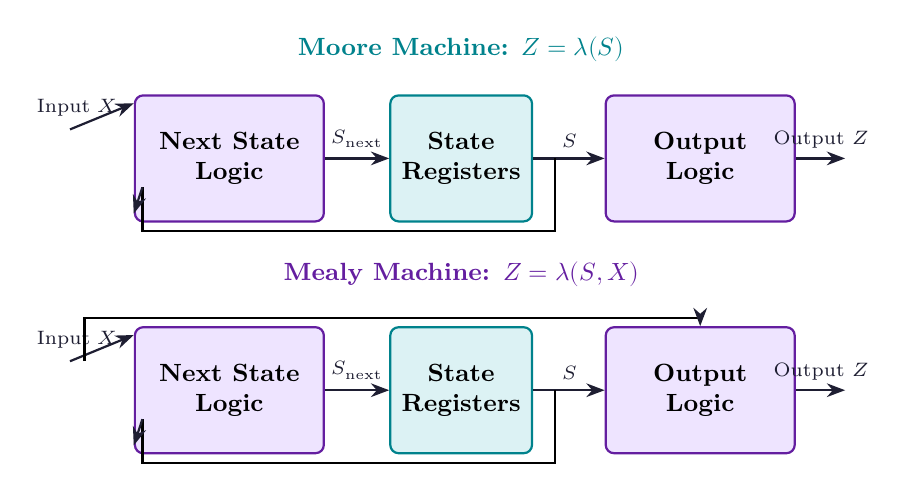
\begin{tikzpicture}[scale=0.92]
  % Moore Machine
  \begin{scope}[yshift=3.2cm]
    \node[combblock] (nsm) at (0,0) {Next State\\Logic};
    \node[ffblock, minimum width=1.8cm, minimum height=1.6cm] (regm) at (3.2,0) {State\\Registers};
    \node[combblock] (outm) at (6.5,0) {Output\\Logic};

    \draw[flowarrow] (-2.2, 0.4) -- (nsm.150) node[pos=0.1, above, font=\scriptsize] {Input $X$};
    \draw[flowarrow] (nsm) -- (regm) node[midway, above, font=\scriptsize] {$S_{\text{next}}$};
    \draw[flowarrow] (regm) -- (outm) node[midway, above, font=\scriptsize] {$S$};
    \draw[flowarrow] (outm) -- (8.5, 0) node[midway, above, font=\scriptsize] {Output $Z$};

    % Feedback
    \draw[thick] (4.5, 0) -- (4.5, -1.0) -- (-1.2, -1.0) -- (-1.2, -0.4);
    \draw[flowarrow] (-1.2, -0.4) -- (nsm.210);

    \node[above, font=\small\bfseries\color{myteal}] at (3.2, 1.2) {Moore Machine: $Z = \lambda(S)$};
  \end{scope}

  % Mealy Machine
  \begin{scope}[yshift=0cm]
    \node[combblock] (nsmy) at (0,0) {Next State\\Logic};
    \node[ffblock, minimum width=1.8cm, minimum height=1.6cm] (regmy) at (3.2,0) {State\\Registers};
    \node[combblock] (outmy) at (6.5,0) {Output\\Logic};

    \draw[flowarrow] (-2.2, 0.4) -- (nsmy.150) node[pos=0.1, above, font=\scriptsize] {Input $X$};
    \draw[flowarrow] (nsmy) -- (regmy) node[midway, above, font=\scriptsize] {$S_{\text{next}}$};
    \draw[flowarrow] (regmy) -- (outmy) node[midway, above, font=\scriptsize] {$S$};
    \draw[flowarrow] (outmy) -- (8.5, 0) node[midway, above, font=\scriptsize] {Output $Z$};

    % Input direct to output logic
    \draw[thick] (-2.0, 0.4) -- (-2.0, 1.0) -- (6.5, 1.0);
    \draw[flowarrow] (6.5, 1.0) -- (outmy.90);

    % Feedback
    \draw[thick] (4.5, 0) -- (4.5, -1.0) -- (-1.2, -1.0) -- (-1.2, -0.4);
    \draw[flowarrow] (-1.2, -0.4) -- (nsmy.210);

    \node[above, font=\small\bfseries\color{mypurple}] at (3.2, 1.3) {Mealy Machine: $Z = \lambda(S, X)$};
  \end{scope}
\end{tikzpicture}
\end{tcolorbox}

\subsection{State Reduction and State Assignment}
\begin{itemize}[leftmargin=*, itemsep=3pt]
  \item \textbf{Equivalent States:} Two states $S_1$ and $S_2$ are equivalent if for every possible input sequence, they produce identical outputs and transition to identical (or equivalent) next states.
  \item \textbf{State Reduction:} Performed using row elimination or the \textbf{Implication Table method} to eliminate redundant states, directly minimizing flip-flop count.
  \item \textbf{State Assignment Techniques:}
    \begin{itemize}
      \item \textbf{Binary Encoding:} Uses minimum number of flip-flops ($n = \lceil\log_2 N\rceil$), requires more combinational decode logic.
      \item \textbf{Gray Encoding:} Consecutive states differ by $1$ bit, minimizing switching noise and power.
      \item \textbf{One-Hot Encoding:} Uses $1$ flip-flop per state ($N$ flip-flops for $N$ states). Maximizes speed and simplifies next-state decode logic; standard choice in FPGA designs.
    \end{itemize}
\end{itemize}

% ===============================================================================
\section{Design of Synchronous Circuits}
% ===============================================================================

\subsection{Sequence Detector / Pulse Train Generator}
A sequence detector inspects an incoming serial binary bit stream and asserts output $Z = 1$ whenever a specific target pattern (e.g., $1011$) is recognized.
\begin{itemize}[leftmargin=*, itemsep=3pt]
  \item \textbf{Overlapping Sequence Detection:} The final bit(s) of a detected sequence can serve as the prefix of the next sequence. For $1011$ with input $1011011 \dots$, two detections occur.
  \item \textbf{Non-Overlapping Sequence Detection:} The detector resets to the initial state upon finding the sequence; subsequent detection starts afresh.
\end{itemize}

\subsection{Pseudo-Random Binary Sequence (PRBS) Generator}
A PRBS generator produces a deterministic, periodic binary sequence possessing noise-like statistical properties using a \textbf{Linear Feedback Shift Register (LFSR)}.
\begin{itemize}[leftmargin=*, itemsep=3pt]
  \item Constructed from an $n$-stage shift register where the input to the first flip-flop is the XOR sum of specific tap outputs defined by a primitive polynomial:
  \begin{equation}
    P(X) = X^n + c_{n-1} X^{n-1} + \dots + c_1 X + 1
  \end{equation}
  \item \textbf{Maximal-Length Sequence (m-sequence):} When $P(X)$ is primitive, the LFSR cycles through all possible non-zero states:
  \begin{equation}
    L = 2^n - 1
  \end{equation}
  (The all-zero state $00 \dots 0$ must be avoided because $\text{XOR}(0,0) = 0$, causing lock-up).
  \item \textbf{Key Applications:} Spread-spectrum communications (CDMA PN codes), cryptographic stream ciphers, and Built-In Self-Test (BIST) pseudo-random test pattern generators.
\end{itemize}

\newpage
% ===============================================================================
\section{Quick Revision Page}
% ===============================================================================

\begin{tcolorbox}[formulabox, title={\textbf{Key Sequential Formulas and Equations at a Glance}}]
\begin{itemize}[leftmargin=*, itemsep=2.5pt]
  \item \textbf{SR Flip-Flop Equation:} $Q_{n+1} = S + \overline{R} Q_n \quad (S \cdot R = 0)$
  \item \textbf{JK Flip-Flop Equation:} $Q_{n+1} = J \overline{Q}_n + \overline{K} Q_n$
  \item \textbf{D Flip-Flop Equation:} $Q_{n+1} = D$
  \item \textbf{T Flip-Flop Equation:} $Q_{n+1} = T \oplus Q_n$
  \item \textbf{Race-Around Condition:} $t_{pd} < t_w < T/2 \quad (J=K=1)$
  \item \textbf{Ripple Counter Maximum Delay:} $t_{\text{total}} = n \cdot t_{pd} \implies f_{\text{max}} = 1/(n \cdot t_{pd})$
  \item \textbf{Ring Counter States:} $N = n \quad (n\text{-bit shift register})$
  \item \textbf{Johnson Counter States:} $N = 2n \quad (n\text{-bit shift register})$
  \item \textbf{Maximal LFSR / PRBS Period:} $L = 2^n - 1$
\end{itemize}
\end{tcolorbox}

\begin{tcolorbox}[defbox, title={\textbf{One-Line Definitions}}]
\begin{itemize}[leftmargin=*, itemsep=2.5pt]
  \item \textbf{Setup Time ($t_s$):} Minimum interval data must remain stable before the active clock edge.
  \item \textbf{Hold Time ($t_h$):} Minimum interval data must remain stable after the active clock edge.
  \item \textbf{Race-Around Condition:} Repeated uncontrolled toggling of a level-triggered JK flip-flop during clock high when $t_{pd} < t_w$.
  \item \textbf{Moore Machine:} A finite state machine whose output is strictly a function of current state only.
  \item \textbf{Mealy Machine:} A finite state machine whose output depends simultaneously on current state and current inputs.
  \item \textbf{Johnson Counter:} An inverted feedback shift register producing $2n$ states for $n$ flip-flops.
\end{itemize}
\end{tcolorbox}

\begin{tcolorbox}[exambox, title={\textbf{Frequently Asked / Viva Questions}}]
\begin{enumerate}[label=\textbf{Q\arabic*.}, leftmargin=*]
  \item \Q{What is the difference between a latch and a flip-flop?}
    A latch is level-triggered (transparent whenever clock/enable is active), whereas a flip-flop is edge-triggered (samples and locks data strictly on clock transition edges).
  \item \Q{Explain the race-around condition in a JK flip-flop. How is it eliminated?}
    When $J=K=1$ in a level-triggered JK FF, if pulse width $t_w > t_{pd}$, the output toggles multiple times before the clock drops, leaving an uncertain final state. It is eliminated by using edge triggering or a Master-Slave configuration.
  \item \Q{Why is Master-Slave JK flip-flop pulse-triggered rather than edge-triggered?}
    Because the master accepts data while the clock is high, and data transfers to the slave on the falling edge; output changes only once per complete clock period.
  \item \Q{How do you convert a JK flip-flop into a D flip-flop?}
    Connect input $D$ directly to $J$, and connect an inverted $D$ ($\overline{D}$) to $K$ ($J = D, K = \overline{D}$).
  \item \Q{What is the propagation delay limitation of ripple counters?}
    Carries must ripple through each stage sequentially ($t = n \cdot t_{pd}$), which limits the maximum clock frequency and creates transient false decoding spikes (glitches).
  \item \Q{Compare Ring counter and Johnson counter for an $n$-bit shift register.}
    A ring counter yields $n$ states and requires no decoding gates. A Johnson counter yields $2n$ states and requires simple 2-input AND gates for decoding.
  \item \Q{What are the key architectural differences between Mealy and Moore FSMs?}
    In a Moore machine, output depends solely on current state ($Z = \lambda(S)$); in a Mealy machine, output depends on both current state and inputs ($Z = \lambda(S, X)$).
  \item \Q{Why does a Mealy machine typically require fewer states than a Moore machine?}
    Because Mealy outputs can vary immediately within a state based on different inputs, whereas a Moore machine requires distinct states for distinct output combinations.
  \item \Q{What is meant by One-Hot state assignment?}
    An encoding scheme using $N$ flip-flops for $N$ states where exactly one flip-flop is high ('1') at any time. It minimizes combinational decoding delay and is optimal for FPGAs.
  \item \Q{What is an LFSR and why can the all-zero state not be used?}
    A Linear Feedback Shift Register uses XOR taps to generate pseudo-random sequences. If all flip-flops become $0$, $\text{XOR}(0,0)=0$, locking the register in permanent zeros.
  \item \Q{What is metastability in digital circuits?}
    A condition where a flip-flop's output hovers at an undefined intermediate voltage level between logic $0$ and $1$ for an indeterminate duration due to a setup/hold time violation.
  \item \Q{How does an overlapping sequence detector differ from a non-overlapping one?}
    An overlapping detector allows the trailing bits of a detected sequence to be reused as the leading bits of the subsequent sequence, producing more output pulses.
\end{enumerate}
\end{tcolorbox}

\begin{tcolorbox}[tikzbox, title={Comparison: Ripple vs. Synchronous Counters and Mealy vs. Moore FSM}]
\centering
\begingroup
\footnotesize
\setlength{\tabcolsep}{3.5pt}
\setlength{\extrarowheight}{2.5pt}
\renewcommand{\arraystretch}{1.35}
\begin{tabularx}{\linewidth}{|B{2.2cm}|Y|Y|Y|}
\hline
\textbf{Category} & \textbf{Architecture A} & \textbf{Architecture B} & \textbf{Key Design Trade-off} \\
\hline
Counter Clocking & \textbf{Ripple Counter:} Flip-flops clocked by previous output & \textbf{Synchronous Counter:} All flip-flops clocked simultaneously & Ripple uses simpler wiring but has high cumulative delay; Synchronous achieves maximum speed. \\
\hline
FSM Output Logic & \textbf{Moore Machine:} $Z = \lambda(S)$ (State only) & \textbf{Mealy Machine:} $Z = \lambda(S, X)$ (State \& Input) & Moore is glitch-free and simpler; Mealy responds 1 cycle faster with fewer states. \\
\hline
Shift Register Counting & \textbf{Ring Counter:} $N = n$ states, uncomplemented loop & \textbf{Johnson Counter:} $N = 2n$ states, inverted loop & Johnson provides double the count states with minimal decoding hardware. \\
\hline
\end{tabularx}
\endgroup
\end{tcolorbox}

\end{document}
